\item ''By giving him the last............of the cake, you will ensure lasting............in our house today''. The words that best fill the blanks in the above sentence are
\begin{enumerate}
\item peas, piece
\item piece, peace
\item peace, piece
\item peace, peas
\end{enumerate}

\item ''Even though there is a vast scope for its........,tourism has remained a/an...........area''. The words that best fill the blanks in the above sentence are
\begin{enumerate}
\item improvement, neglected
\item rejection, approved
\item fame, glum
\item interest, disinterested
\end{enumerate} 

\item If the number $715k423$ is divisible by 3($k$ denotes the missing digit in the thousandths place), then the smallest whole number in the place of $k$ is...............
\begin{enumerate}
\item 0
\item 2
\item 5
\item 6
\end{enumerate}

\item What is the value of 
\begin{align*}
1 + \frac{1}{4} + \frac{1}{16} + \frac{1}{64} + \frac{1}{256} + ........?
\end{align*}
\begin{enumerate}
\item 2
\item 7/4
\item 3/2
\item 4/3
\end{enumerate}

\item A 1.5m tall person is standing at a distance of 3m from a lamp post. The light from the lamp at the top of the post casts her shadow. The length of the shadow is twice her height. What is the height of the lamp post in meters?
\begin{enumerate}
\item 1.5
\item 3
\item 4.5
\item 6
\end{enumerate}

\item Leila aspires to buy a car woth Rs. 10,00,000 after 5 years. What is the minimum amount in Rupees that she should deposit now in a bank which offers $10\%$ annual rate of interest, if the interest was compounded annually?
\begin{enumerate}
\item 5,00,000
\item 6,21,000
\item 6,66,667
\item 7,50,000
\end{enumerate}

\item Two alloys A and B contain gold and copper in the ratios of 2:3 and 3:7 by mass, respectively. Equal masses of alloys A and B are melted to make an alloy C. The ratio of gold to copper in alloy C is
\begin{enumerate}
\item 5:10
\item 7:13
\item 6:11
\item 9:13
\end{enumerate}

\item The Cricket Board has long recognized John's potential as a leader of the team. However, his on-field temper has always been a matter of concern for them since his junior days. While this aggression has filled stadia with die-hard fans, it has taken a toll on his own batting. Until recently, it appeared that he found it difficult to convert his aggression into big scores. Over the past three seasons though, that picture of John has been replaced by a cerebral, calculative and successful batsman-captain. After many years, it appears that the team has finally found a complete captain. Which of the following statements can be logically inferred from the above paragraph?\\
(i) Even as a junior cricketer, John was considered a good captain.\\
(ii) Finding a complete captain is a challenge.\\
(iii) Fans and the Cricket Board have differing views on what they want in a captain.\\
(iv) Over the past three seasons John has accumulated big scores.
\begin{enumerate}
\item (i), (ii) and (iii) only
\item (iii) and (iv) only
\item  (ii) and (iv) only
\item (i), (ii), (iii) and (iv)
\end{enumerate}

\item A cab was involved in a hit and run accident at night. You are given the following data about the cabs in the city and the accident.\\
(i) $85\%$ percentage of cabs in the city are green and the remaining cabs are blue.\\
(ii) A witness identified the cab involved in the accident as blue.\\
(iii) It is known that a witness can correctly identify the cab colour only $80\%$ percentage of the time.\\
Which of the following options is closest to the probability that the accident was caused by a blue cab?
\begin{enumerate}
\item $12\%$ 
\item $15\%$
\item $41\%$
\item $80\%$
\end{enumerate}

\item A coastal region with unparalleled beauty is home to many species of animals. It is dotted with coral reefs and unspoilt white sandy beaches. It has remained inaccessible to tourists due to poor connectivity and lack of accommodation. A company has spotted the opportunity and is planning to develop a luxury resort with helicopter service to the nearest major city airport. Environmentalists are upset that this would lead to the region becoming crowded and polluted like any other major beach resorts.\\
Which one of the following statements can be logically inferred from the information given in the above paragraph?
\begin{enumerate}
\item The culture and tradition of the local people will be influenced by the tourists.
\item The region will become crowded and polluted due to tourism.
\item The coral reefs are on the decline and could soon vanish.
\item Helicopter connectivity would lead to an increase in tourists coming to the region.
\end{enumerate}

\item Two identical nMOS transistors $M_1$ and $M_2$ are connected as shown below. The circuit is used as an amplifier with the input connected between $G$ and $S$ terminals and the output taken between $D$ and $S$ terminals. $V_bias$ and 
$V_D$ are so adjusted that both transistors are in saturation. The transconductance of this combination is defined as 
$g_m = \frac{\partial i_D}{\partial v_{GS}}$ while the output resistance is $r_o = \frac{\partial v_{DS}}{\partial i_D}$, where $i_D$ is the current flowing into the drain of $M_2$. Let $g_{m1}$, $g_m2$ be the transconductances and $r_{o1}$, 
$r_{o2}$ be the output resistances of transistors $M_1$ and $M_2$, respectively.

Which of the following statements about estimates for $g_m$ and $r_o$ is correct?

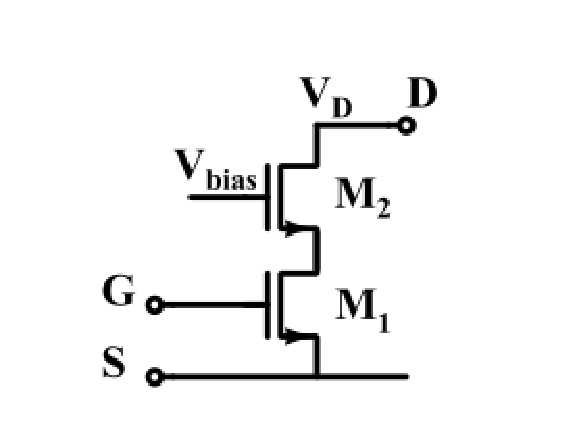
\includegraphics[scale=0.65]{11}

\begin{enumerate}
\item $g_m \approx g_{m1}.g_{m2}.r_{o2}$ and $r_o \approx r_{o1} + r_{o2}$
\item $g_m \approx g_{m1} + g_{m2}$ and $r_o \approx r_{o1} + r_{o2}$
\item $g_m \approx g_{m1}$ and $r_o \approx r_{o1}.g_{m2}.r_{o2}$
\item $g_m \approx g_{m1}$ and $r_o \approx r_{o2}$
\end{enumerate} 

\item In the circuit shown below, the op-amp is ideal and Zener voltage of the diode is 2.5 volts. At the input, unit step voltage is applied, i.e. $v_{IN}(t) = u(t)$volts. Also, at t = 0, the voltage across each of the capacitor is zero.

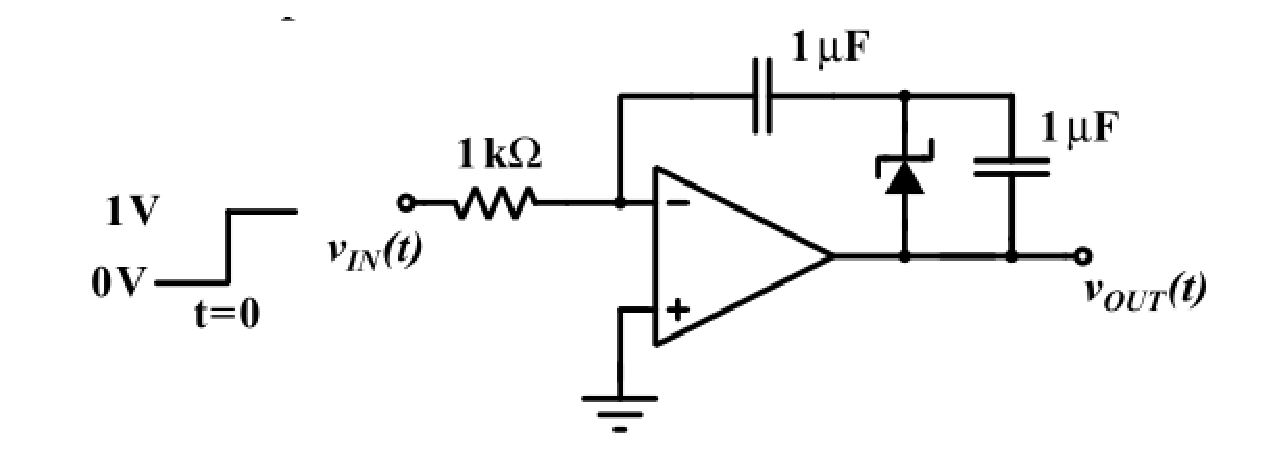
\includegraphics[scale=0.35]{12}

The time t, in milliseconds, at which the output voltage $v_{OUT}$ crosses $-10V$ is
\begin{enumerate}
\item 2.5
\item 5
\item 7.5
\item 10
\end{enumerate}

\item A good transimpedance amplifier has
\begin{enumerate}
\item low input impedance and high output impedance
\item high input impedance and high output impedance
\item high input impedance and low output impedance
\item low input impedance and low output impedance
\end{enumerate}

\item Let the input be $u$ and the output be $y$ of a system, and the other parameters are real constants. Identify which among the following systems is not a linear system.
\begin{enumerate}
\item $\frac{d^3y}{dt^3} + a_1\frac{d^2y}{dt^2} + a_2\frac{dy}{dt} + a_3y = b_3u + b_2\frac{du}{dt} + b_1\frac{d^2u}{dt^2}$
\item $y(t) = \int_{0}^{t}e^{\alpha(t - \tau)}\beta u(\tau)d\tau$
\item $y = au + b$, $b \neq 0$
\item $y = au$
\end{enumerate}

\item The Nyquist stability criterion and the Routh criterion both are powerful analysis tools for determining the stability of feedback controllers. Identify which of the following statements is FALSE.
\begin{enumerate}
\item Both the criteria provide information relative to the stable gain range of the system.
\item The general shape of the Nyquist plot is readily obtained from the Bode magnitude plot for all minimum-phase systems.
\item The Routh criterion is not applicable in the condition of transport lag, which can be readily handled by the Nyquist criterion.
\item The closed-loop frequency response for a unity feedback system cannot be obtained from the Nyquist plot.
\end{enumerate}

\item Consider 
\begin{align*}
p(s) = s^3 + a_2s^2 + a_1s + a_0
\end{align*}
with all real coefficients. It is known that its derivative $p'(s)$ has no real roots of $p(s)$ is
\begin{enumerate}
\item 0
\item 1
\item 2
\item 3
\end{enumerate}

\item In a p-n junction diode at equilibrium, which one of the following statements is $NOT$ true?
\begin{enumerate}
\item The hole and electron diffusion current components are in the same direction.
\item The hole and electron drift current components are in the same direction.
\item On an average, holes and electrons drift in opposite direction.
\item On an average, electrons drift and diffusion in same direction.
\end{enumerate}

\item The logic function $f(X, Y)$ realized by the given circuit is

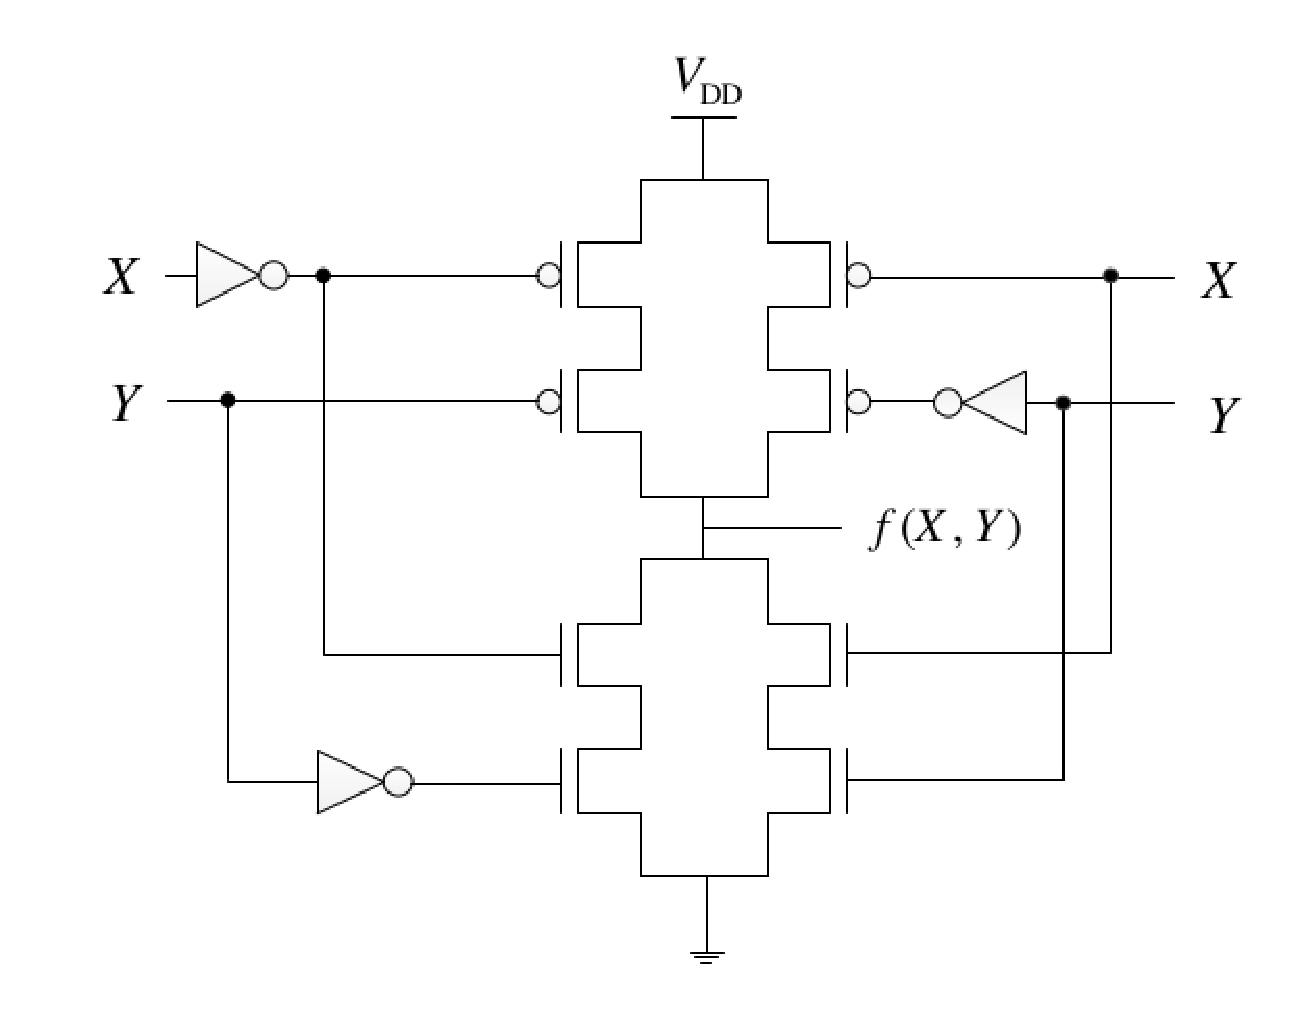
\includegraphics[scale=0.35]{18}

\begin{enumerate}
\item NOR
\item AND
\item NAND
\item XOR
\end{enumerate}

\item A function $F(A, B, C)$ defined by three Boolen variables A, B and C when expressed as sum of products is given by
\begin{align*}
F = \bar{A}.\bar{B}.\bar{C} + \bar{A}.B.\bar{C} + A.B.\bar{C}
\end{align*}
where $\bar{A}$, $\bar{B}$ and $\bar{C}$ are the components of the respective variables. The product of sums(POS) form of the function F is
\begin{enumerate}
\item $F = (A + B + C).(A + \bar{B} + C).(\bar{A} + B + C)$
\item $F = (\bar{A} + \bar{B} + \bar{C}).(\bar{A} + B + \bar{C}).(A + \bar{B} + \bar{C})$
\item $F = (A + B + \bar{C}).(A + \bar{B} + \bar{C}).(\bar{A} + B + \bar{C}).(\bar{A} + \bar{B} + C).(\bar{A} + \bar{B} + \bar{C})$
\item $F = (\bar{A} + \bar{B} + C).(\bar{A} + B + C).(A + \bar{B} + C).(A + B + \bar{C}).(A + B + C)$
\end{enumerate}

\item The P, Q and R shown on the Smith chart(normalized impedance chart) in the following figure represent.

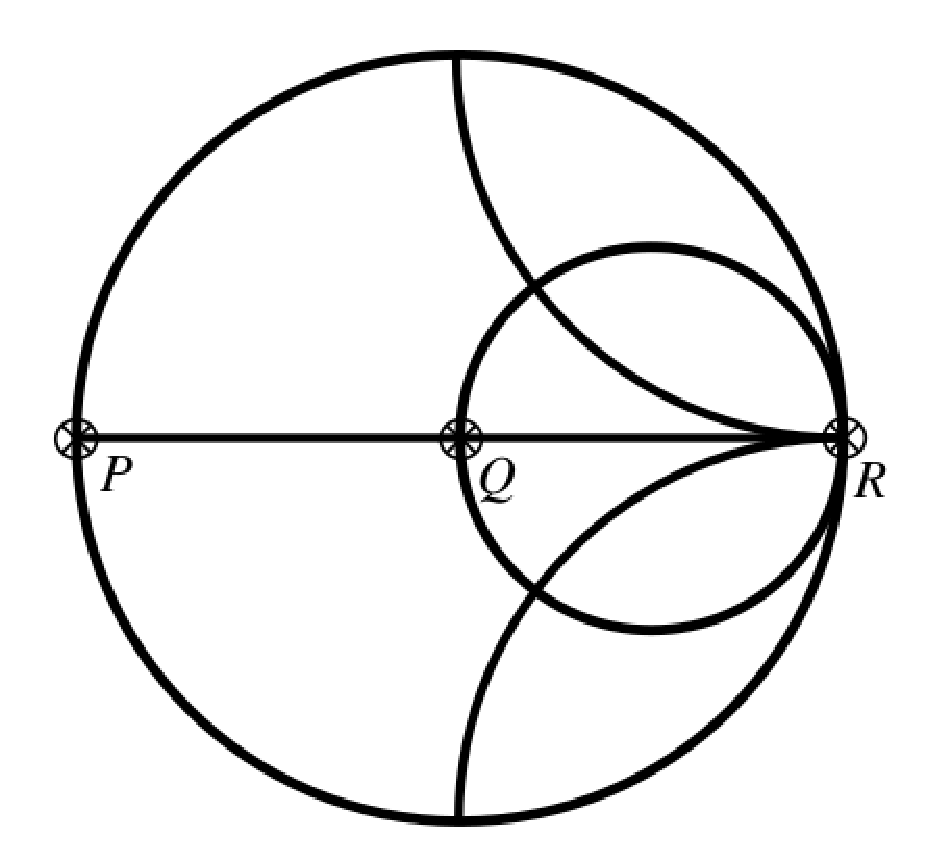
\includegraphics[scale=0.3]{20}

\begin{enumerate}
\item P: Open Circuit, Q: Short Circuit, R: Matched Load
\item P: Open Circuit, Q: Matched Load, R: Shirt Circuit
\item P: Short Circuit, Q: Matched Load, R: Open Circuit
\item P: Short Circuit, Q: Open Circuit, R: Matched Load
\end{enumerate}

\item Let $M$ be a real $4 \times 4$ matrix. Consider the following statements:\\
S1: $M$ has 4 linearly independent eigenvectors\\
S2: $M$ has 4 distinct eigenvalues\\
S3: $M$ is non-singular\\
Which one among the following is TRUE?
\begin{enumerate}
\item S1 implies S2
\item S1 implies S3
\item S2 implies S1
\item S3 implies S2
\end{enumerate}

\item Let 
\begin{align*}
f(x, y) = \frac{ax^2 + by^2}{xy}
\end{align*}
where a and b are constants. If $\frac{\partial f}{\partial x} = \frac{\partial f}{\partial y}$ at x = 1 and y = 2, then the relation between a and b is
\begin{enumerate}
\item $a = \frac{b}{4}$
\item $a = \frac{b}{2}$
\item $a = 2b$
\item $a = 4b$
\end{enumerate}

\item A discrete-time all-pass system has two of its poles at $0.25\angle 0^{o}$ and $2\angle 30^{o}$. Which one of the following statements about the system is TRUE?
\begin{enumerate}
\item It has two more poles at $0.5 \angle 30^{o}$ and $4 \angle 0^{o}$.
\item It is stable only when the impulse response is two-sided.
\item It has constant phase response over all frequencies.
\item It has constant phase response over the entire z-plane
\end{enumerate}

\item Let $x(t)$ be a periodic function with period T = 10. The fourier series coefficents for this series are denoted by $a_k$, that is
\begin{align*}
\sum_{k = -\infty}^{\infty}a_ke^{jk\frac{2\pi}{T}t}
\end{align*}
The same function $x(t)$ can also be considered as a periodic function with period $T" = 40$. Let $b_k$ be the Fourier series coefficients when period is taken as $T'$. If $\sum_{k = \infty}^{\infty}|a_k| = 16$, then $\sum_{k = \infty}^{\infty}|b_k|$ is equal to
\begin{enumerate}
\item 256
\item 64
\item 16
\item 4
\end{enumerate}

\item Consider the following amplitude modulated signal:
\begin{align*}
s(t) = \cos(2000\pi t) + 4\cos(2400\pi t) + \cos(2800\pi t)
\end{align*}
The ratio(accurate to three decimal places) of the power of the message signal to the power of the carrier signal is.........

\item Consider a binary channel code in which each code word has a fixed length of 5 bits. The Hamming distance between any pair of distinct code words in this code is at least 2. The maximum number of codewords such a code can contain is.........

\item A binary source generates symbols $X \in {-1, 1}$ which are transmitted over a noisy channel. The probability of trasmitting $X = 1$ is 0.5. Input to the threshold detector is $R = X + N$. The probability density function $f_N(n)$ of the noise N is shown below.

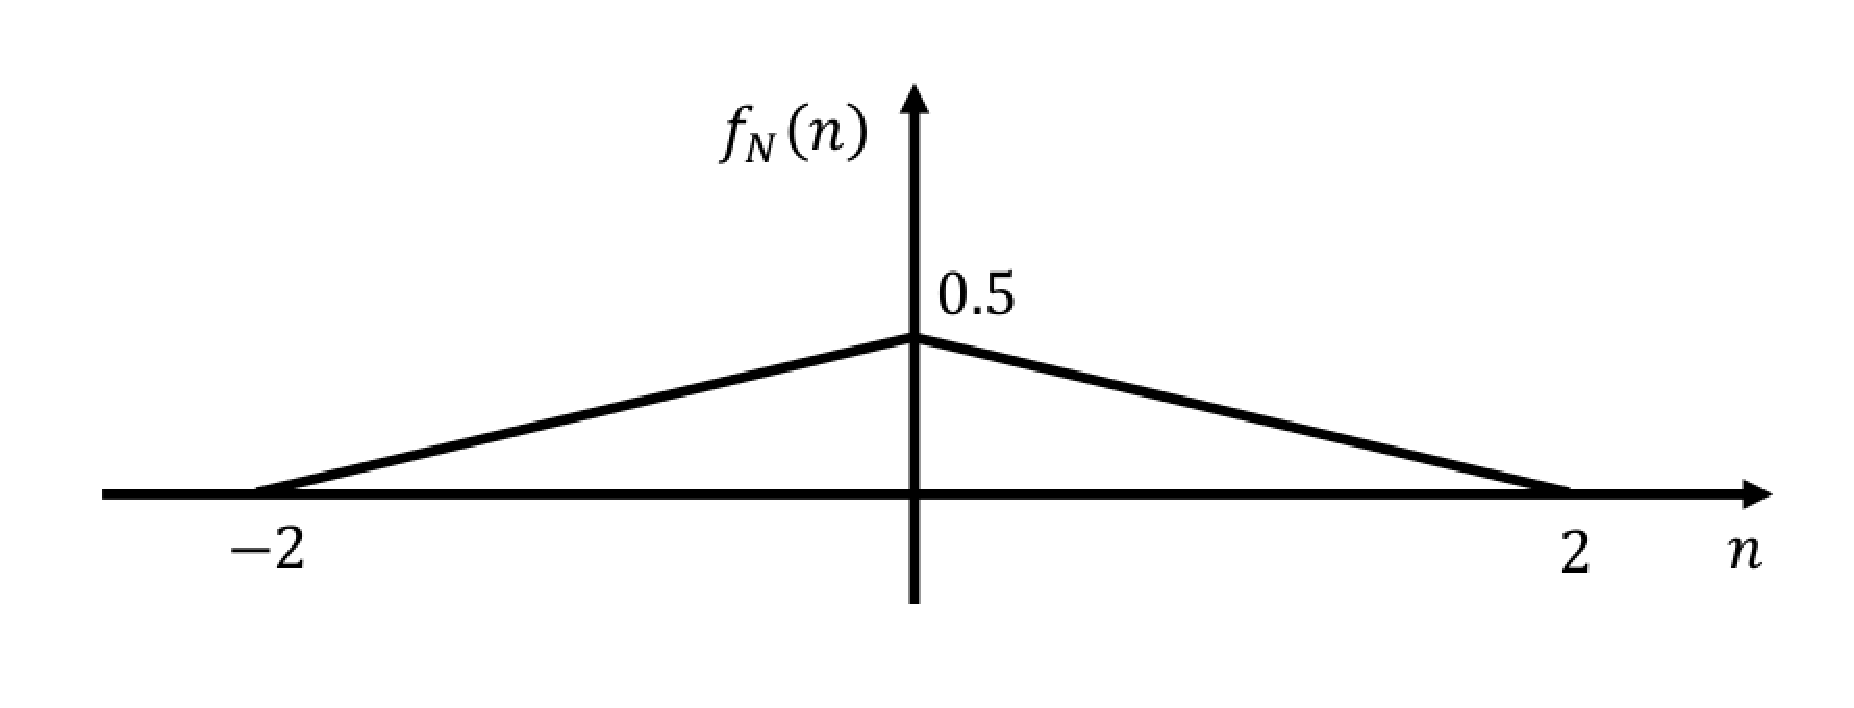
\includegraphics[scale=0.25]{27}

If the detection threshold is zero, then the probability of error(correct to two decimal places) is..........

\item A p-n step junction diode with a contact potential of 0.65V has a depletion width of $1\mu m$ at equilibrium. The forward voltage(in volts, correct to two decimal places) at which this width reduces to $0.6\mu m$ is...........

\item A traffic signal cycles from GREEN to YELLOW, YELLOW to RED and RED to GREEN. In each cycle, GREEN is turned on for 70 seconds, YELLOW is turned on for 5 seconds and the RED is turned on for 75 seconds. This traffic light has to be implemented using a finite state machine(FSM). The only input to this FSM is a clock of 5 second period. The minimum number of flip-flops required to implement thsi FSM is...........

\item There are two photolithography systems: one with light source of wavelength $\lambda_1 = 156nm$ (System 1) and another with light source of wavelength $\lambda_2 = 325nm$ (System 2). Both photolithography systems are otherwise identical. If the minimum feature sizes that can be realized using System-1 and System-2 are $L_{min1}$ and $L_{min2}$ respectively, the ratio $L_{min1}/L_{min2}$ (correct to two decimal places) is...............

\item A lossy transmission line has resistance per unit length $R = 0.05\Omega/m$. The line is distortionless and has characteristic impedance of $50\Omega$. The attenuation constant (in Np/m, correct to three decimal places) of the line is...........

\item Consider matrix 
$A = \begin{bmatrix}
k & 2k \\ k^2 - k & k^2
\end{bmatrix}$ 
and the vector
$x = \begin{bmatrix}
 x_1 \\ x_2
\end{bmatrix}$. 
The number of distinct real values of k for which the equation $Ax = 0$ has infintely many solutions is...........

\item Let $X_1$, $X_2$, $X_3$ and $X_4$ be independent normal random variables with zero mean and unit variance. The probability that $X_4$ is the smallest among the four is.............

\item Taylor series expansion of 
\begin{align*}
f(x) = \int_{0}^{x}e^{-\left(\frac{t^2}{2}\right)}dt
\end{align*}
around x = 0 has the form
\begin{align*}
f(x) = a_0 + a_1x + a_2x^2 +.........
\end{align*}
The coefficient $a_2$(correct to two decimal places) is equal to.............

\item The ABCD matrix for a two-port network is defined by
\begin{align*}
\begin{bmatrix}
V_1 \\ I_1
\end{bmatrix}
=
\begin{bmatrix}
A & B \\ C & D
\end{bmatrix}
\begin{bmatrix}
V_2 \\ -I_2
\end{bmatrix}
\end{align*}

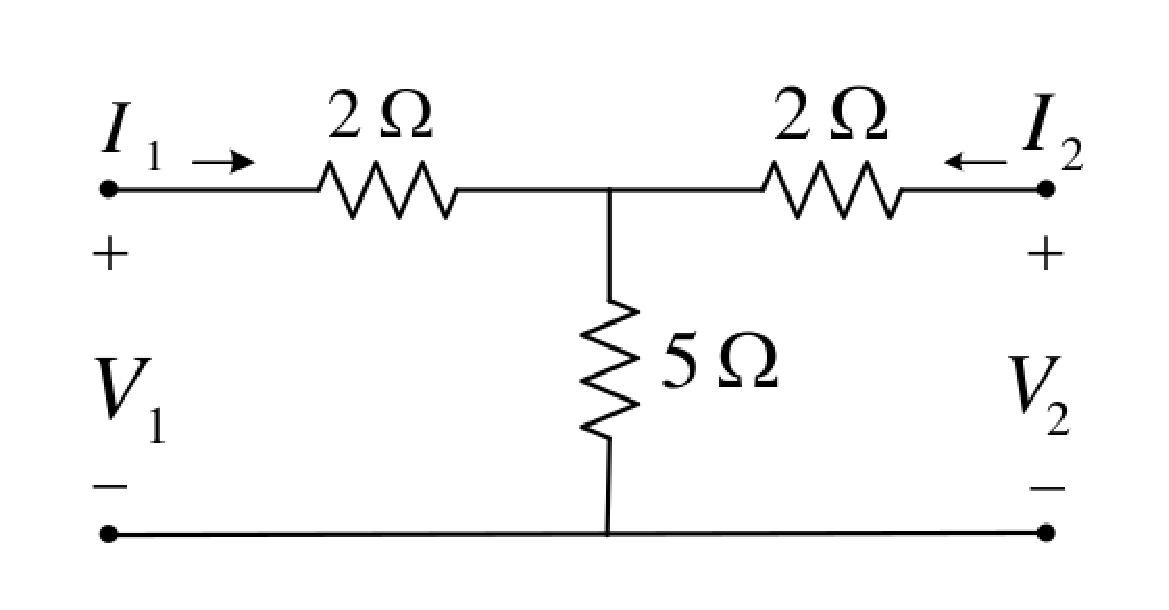
\includegraphics[scale=0.3]{35}

The parameter B for the given two-port network(in ohms, correct to two decimal places) is...........

\item The circiut shown in the figure is used to provide regulated voltage (5V) across the $1k\Omega$ resistor. Assume that the Zener diode has a constant reverse breakdown voltage for a current range, starting form a minimum required Zener current, $I_{Z min} = 2mA$ to its maximum allowable current. The input voltage $V_t$ may vary by $5\%$ from its nominal value of 6V. The resistnace of the diode in the breakdown region is negligible.

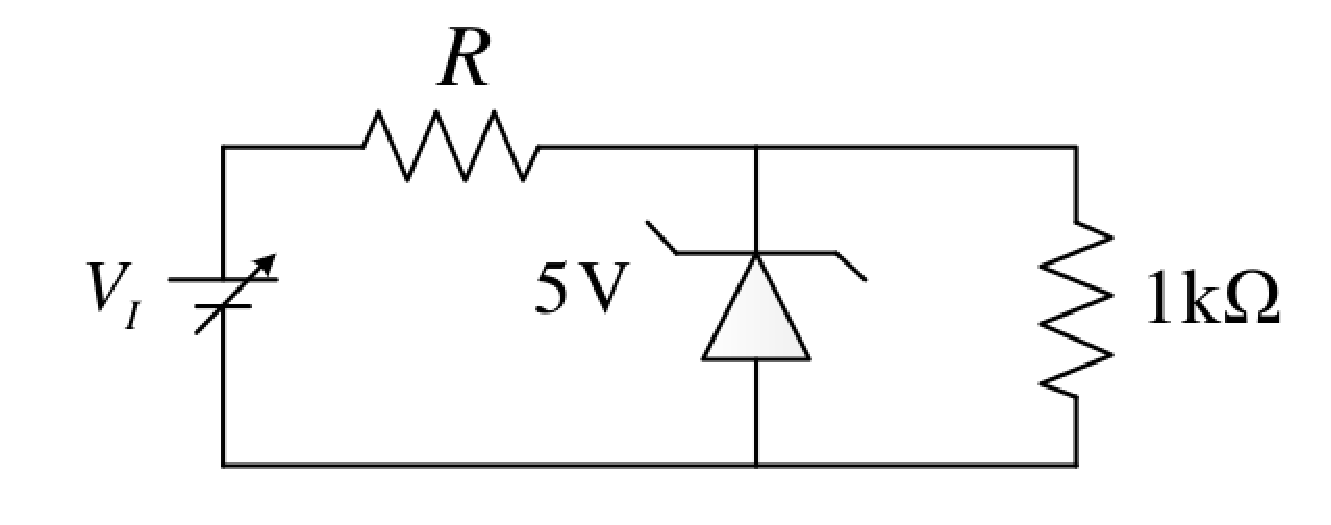
\includegraphics[scale=0.3]{36}

The value of R and the minimum required power dissipation rating of the diode, respectively, are
\begin{enumerate}
\item $186\Omega$ and $10m W$
\item $100\Omega$ and $40m W$
\item $100\Omega$ and $10m W$
\item $186\Omega$ and $40m W$
\end{enumerate}

\item Let $c(t) = A_c \cos(2\pi f_ct)$ and $m(t) = \cos(2\pi f_mt)$. It is given that $f_c >> 5f_m$. The signal $c(t) + m(t)$ is applied to the input of a non-linear device, whose output $v_o(t)$ is related to the input $v_i(t)$ as $v_o(t) = av_i(t) + b_{i}^{2}(t)$, where a and b are positive constants. The output of the non-linear device is passed through an ideal band-pass filter with centre frequency $f_c$ and bandwidth $3f_m$, to produce an amplitude modulated(AM) wave. If it is desired to have the sideband power of the AM wave to be half of the carrier power, then $a/b$ is
\begin{enumerate}
\item 0.25
\item 0.5
\item 1
\item 2
\end{enumerate}

\item Consider a white Gaussian noise process $N(t)$ with two-sided power spectral density $S_N(f) = 0.5W/Hz$ as input to a filter with impulse respense $0.5e^{-t^2/2}$(where t is in seconds) resulting in output $Y(t)$. The power in $Y(t)$ in watts is
\begin{enumerate}
\item 0.11
\item 0.22
\item 0.33
\item 0.44
\end{enumerate}

\item The state equation and the output equation of a control system are given below:
\begin{align*}
\frac{dx}{dt} = 
\begin{bmatrix}
-4 & -1.5 \\ 4 & 0
\end{bmatrix}x + 
\begin{bmatrix}
2 \\ 0
\end{bmatrix}u
\end{align*}
\begin{align*}
y = \begin{bmatrix}
1.5 & 0.625
\end{bmatrix}x
\end{align*}
The trasfer function representation of the system is
\begin{enumerate}
\item $\frac{3s + 5}{s^2 + 4s + 6}$
\item $\frac{3s - 1.875}{s^2 + 4s + 6}$
\item $\frac{4s + 1.5}{s^2 + 4s + 6}$
\item $\frac{6s + 5}{s^2 + 4s + 6}$
\end{enumerate}

\item Red(R), Green(G) and Blue(B) Light Emitting Diodes(LEDs) were fabricated using p-n junctions of three different inorganic semoconductors having different band-gaps. The built-in voltages of red, green and blue diodes are $V_R$, $V_G$ and $V_B$ respecively. Assume donor and acceptor doping to be the same ($N_A$ and $N_D$ respectively) in the p and n sides of all the three diodes.

Which one of the following relationships about the built-in voltages is TRUE?
\begin{enumerate}
\item $V_R > V_G > V_B$
\item $V_R < V_G < V_B$
\item $V_R = V_G = V_B$
\item $V_R > V_G < V_B$ 
\end{enumerate} 

\item A four-variable Boolen function is realized using $4 \times 1$ multiplexers as shown in the figure.

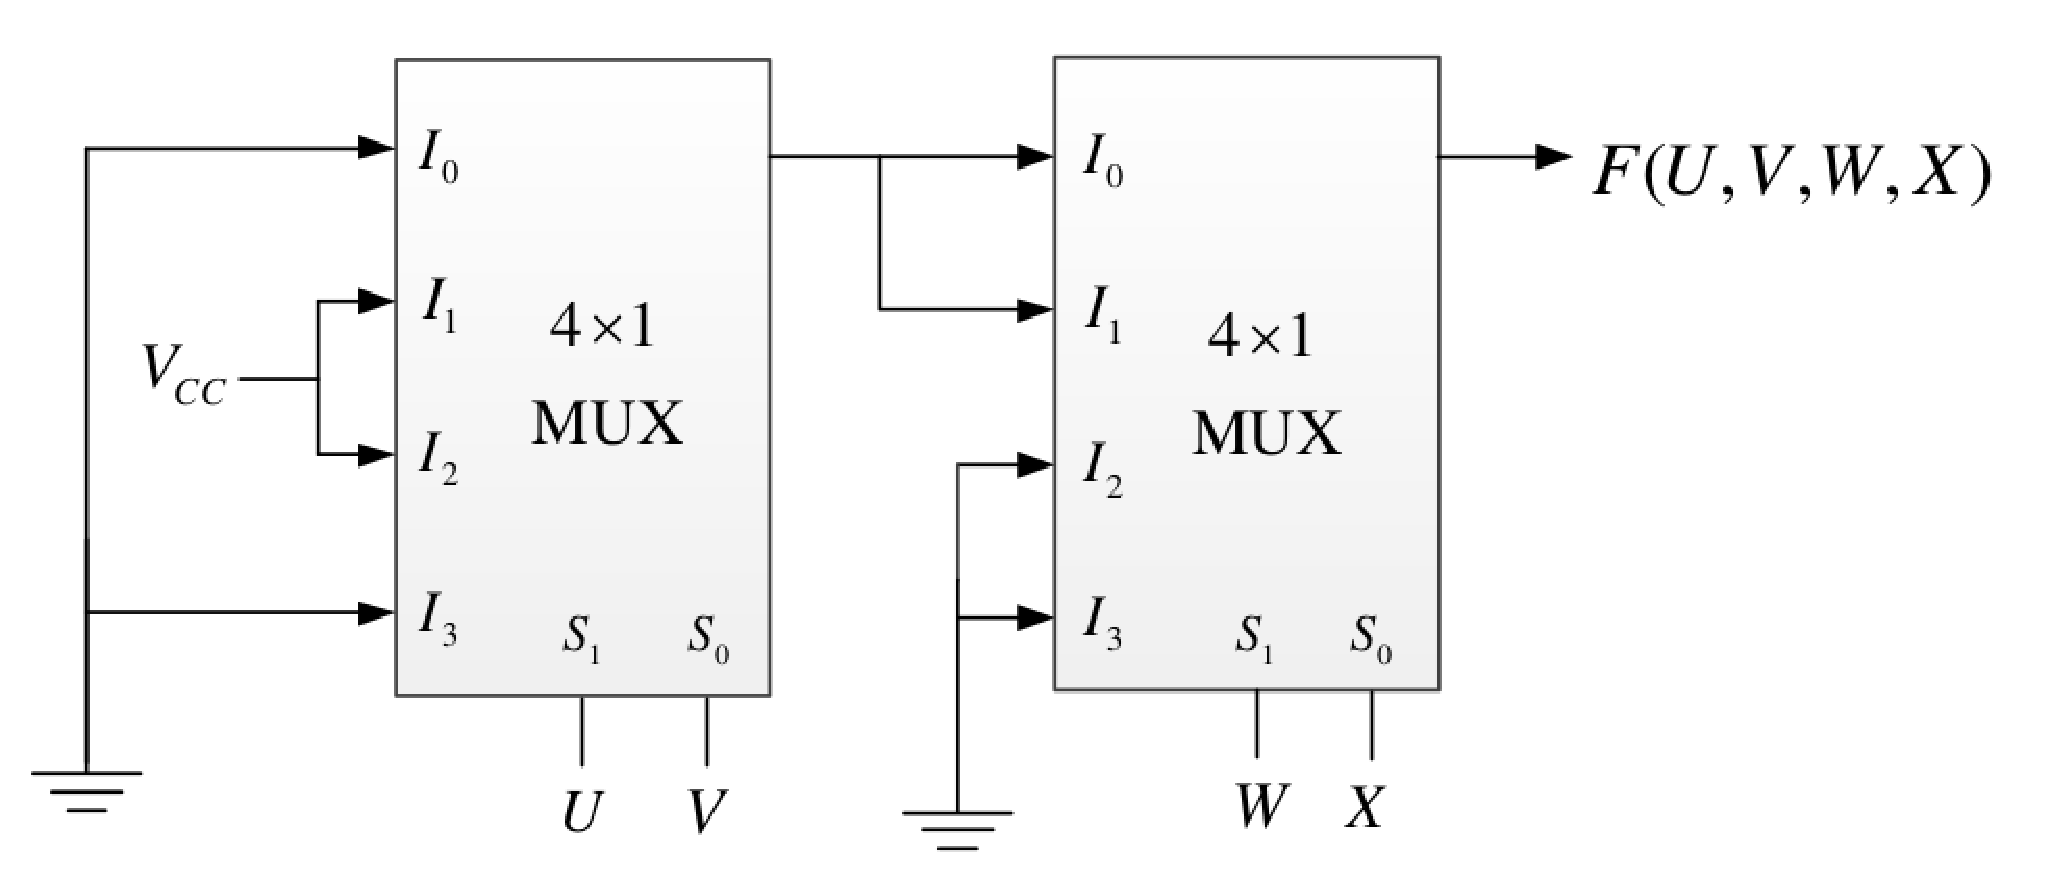
\includegraphics[scale=0.22]{41}

The minimized expression for F(U, V, W, X) is
\begin{enumerate}
\item $(UV + \bar{U}\bar{V})\bar{W}$
\item $(UV + \bar{U}\bar{V})(\bar{W}\bar{X} + \bar{w}X)$
\item $(U\bar{V} + \bar{U}V)\bar{W}$
\item $(U\bar{V} + \bar{U}V)(\bar{W}\bar{X} + \bar{w}X)$
\end{enumerate}

\item A $2 \times 2$ ROM array is built with the help of diodes as shown in the circuit below. Here WO and WI are signals that select the word lines and BO and B1 are signals that that are output of the sense amps based on the stored data corresponding to the bit lines during the read operation.

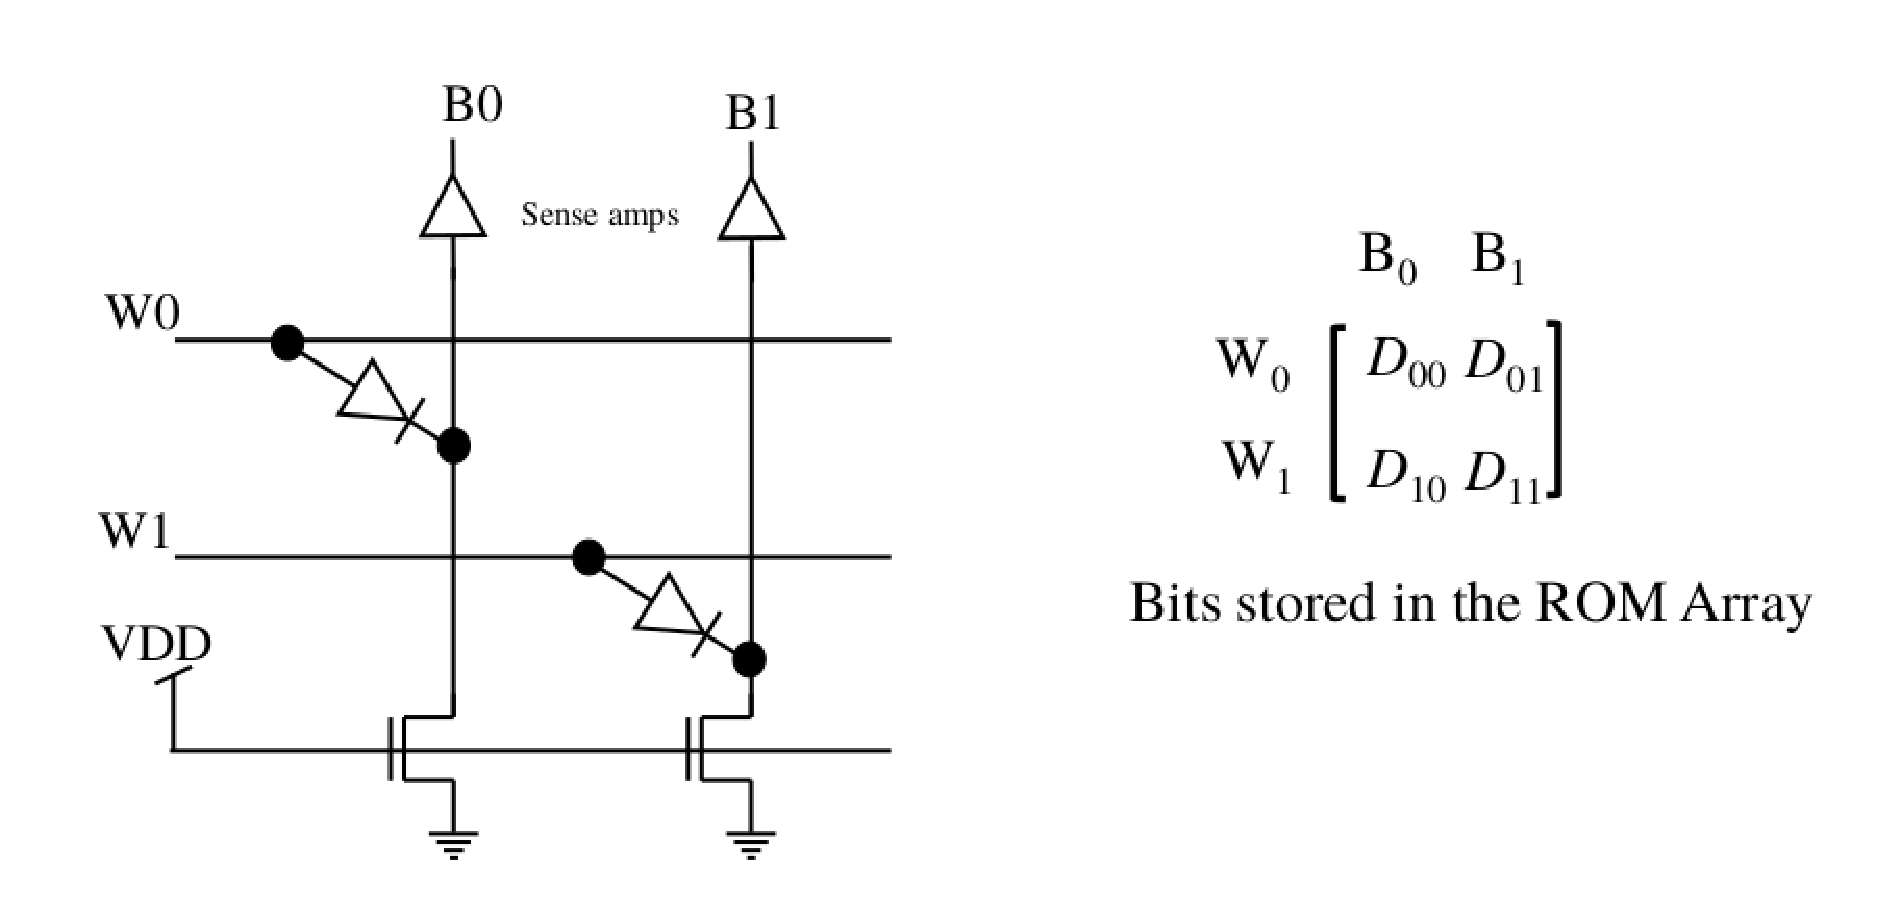
\includegraphics[scale=0.22]{42}

During the read operation, the selected word line goes high and the other word line is in a high impedance state. As per the implementation show in the circuit diagram above, what are the bits correspinding to $D_{ij}$(where i = 0 or j = 0 or 1) stored in the ROM?
\begin{enumerate}
\item $\begin{bmatrix}
1 & 0 \\ 0 & 1
\end{bmatrix}$
\item $\begin{bmatrix}
0 & 1 \\ 1 & 0
\end{bmatrix}$
\item $\begin{bmatrix}
1 & 0 \\ 1 & 0
\end{bmatrix}$
\item $\begin{bmatrix}
1 & 1 \\ 0 & 0
\end{bmatrix}$
\end{enumerate}

\item The distance (in meters) a wave has to propagate in a medium having a skin depth of 0.1m so that the amplitude of the wave attenuates by 20dB, is
\begin{enumerate}
\item 0.12
\item 0.23
\item 0.46
\item 2.3
\end{enumerate}

\item A curve passes through the point (x = 1, y = 0) and satisfies the differential equation
\begin{align*}
\frac{dy}{dx} = \frac{x^2 + y^2}{2y} + \frac{y}{x}
\end{align*}
The equation that describes the curve is
\begin{enumerate}
\item $ln\left(1 + \frac{y^2}{x^2}\right) = x - 1$
\item $\frac{1}{2} ln\left(1 + \frac{y^2}{x^2}\right) = x - 1$
\item $ln\left(1 + \frac{y}{x}\right) = x - 1$
\item $\frac{1}{2} ln\left(1 + \frac{y}{x}\right) = x - 1$
\end{enumerate}

\item For the circuit given in the figure, the voltage $V_c$(in volts) across the capacitor is

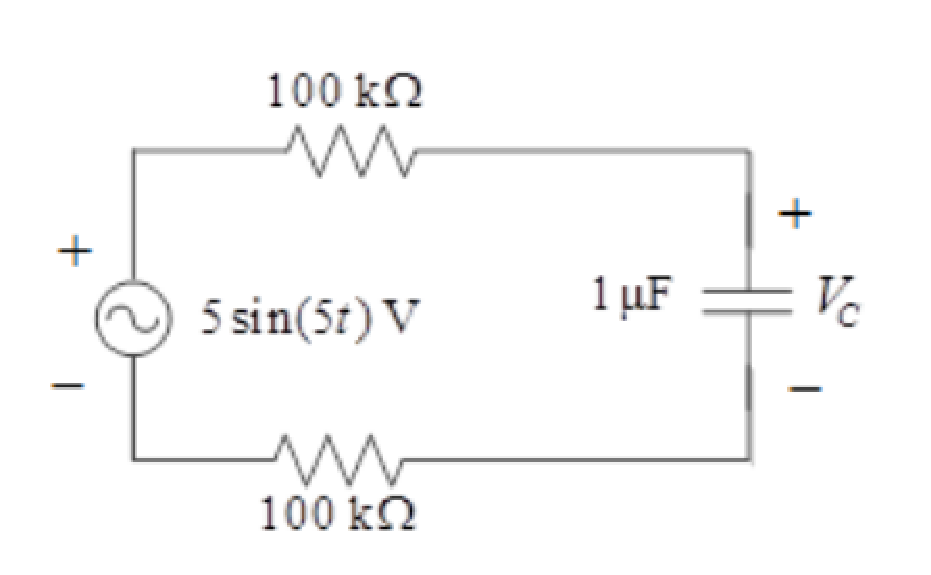
\includegraphics[scale=0.4]{45}

\begin{enumerate}
\item $1.25\sqrt{2}\sin(5t - 0.25\pi)$
\item $1.25\sqrt{2}\sin(5t - 0.125\pi)$
\item $2.5\sqrt{2}\sin(5t - 0.25\pi)$
\item $2.5\sqrt{2}\sin(5t - 0.125\pi)$
\end{enumerate}

\item For the circuit given in the figure, the magnitude of the loop current(in amperes, correct to three decimal places) 0.5 second after closing the switch is........

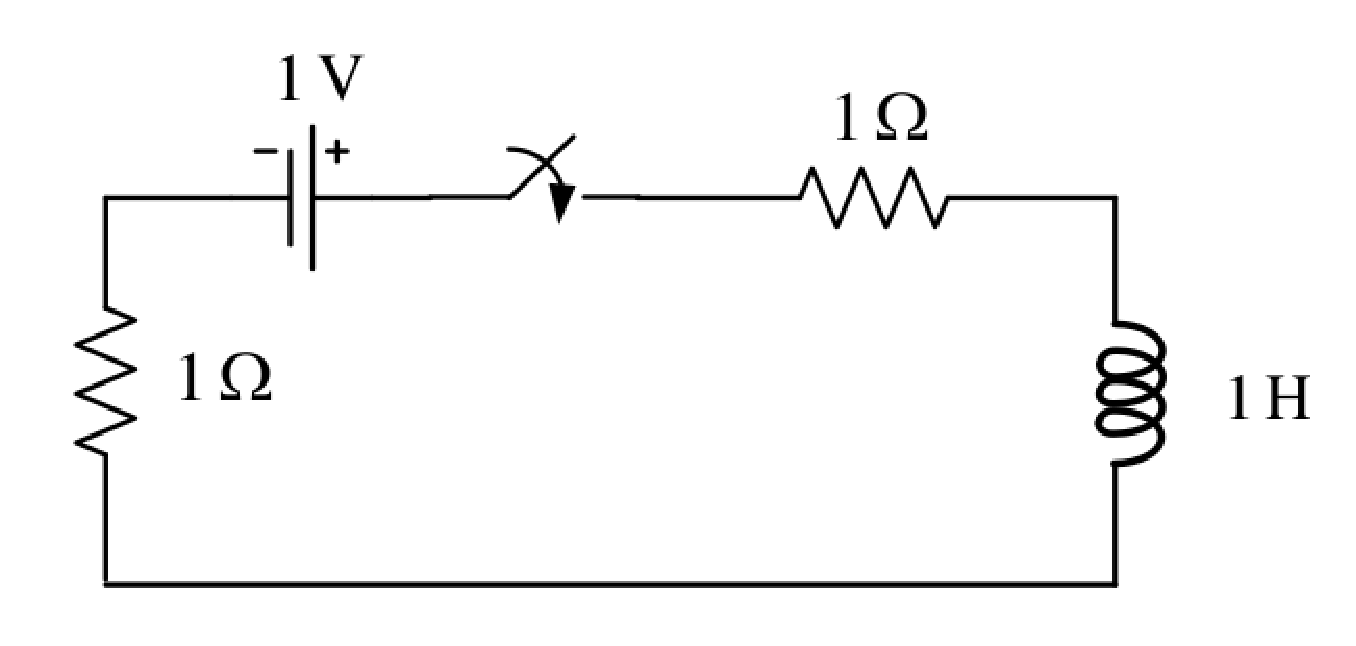
\includegraphics[scale=0.3]{46}

\item A dc current of $26\mu A$ flows through the circiut shown. The diode circuit is forwarded biased and it has an ideality factor of one. At the quiescent point, the diode has a junction capacitance of 0.5nF. Its neutral region resistances can be neglected. Assume that the room temperature thrmal equivalent voltage is 26mV.

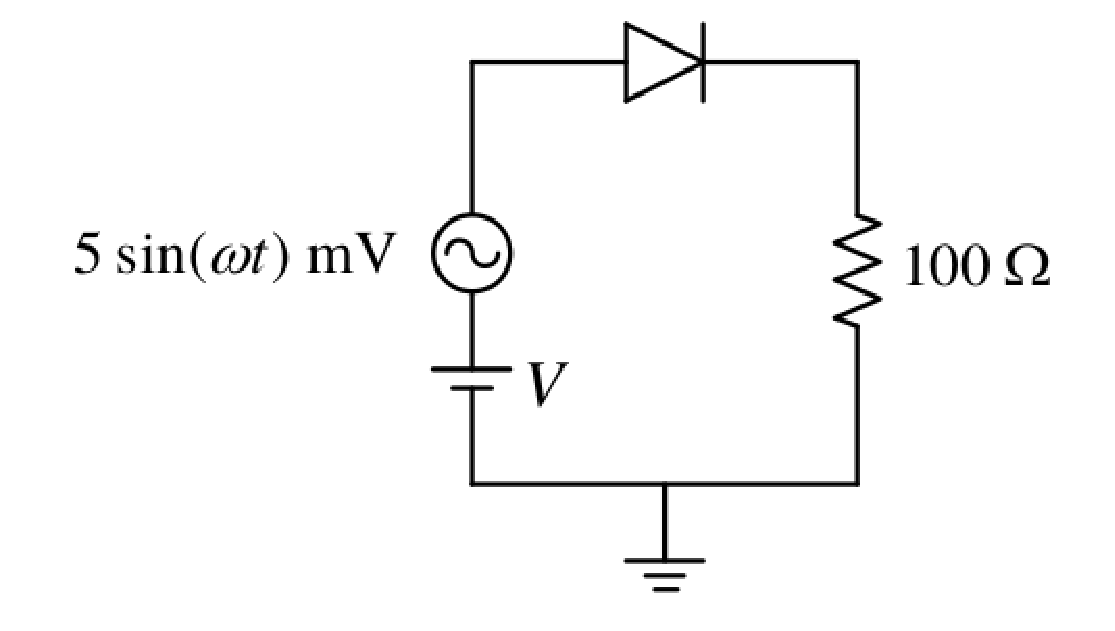
\includegraphics[scale=0.35]{47}

For $\omega = 2 \times 10^{6}rad/s$, the amplitude of the small-signal component of diode current(in $\mu A$, correct to one decimal place) is...........

\item An op-amp based circuit is implemented as shown below.

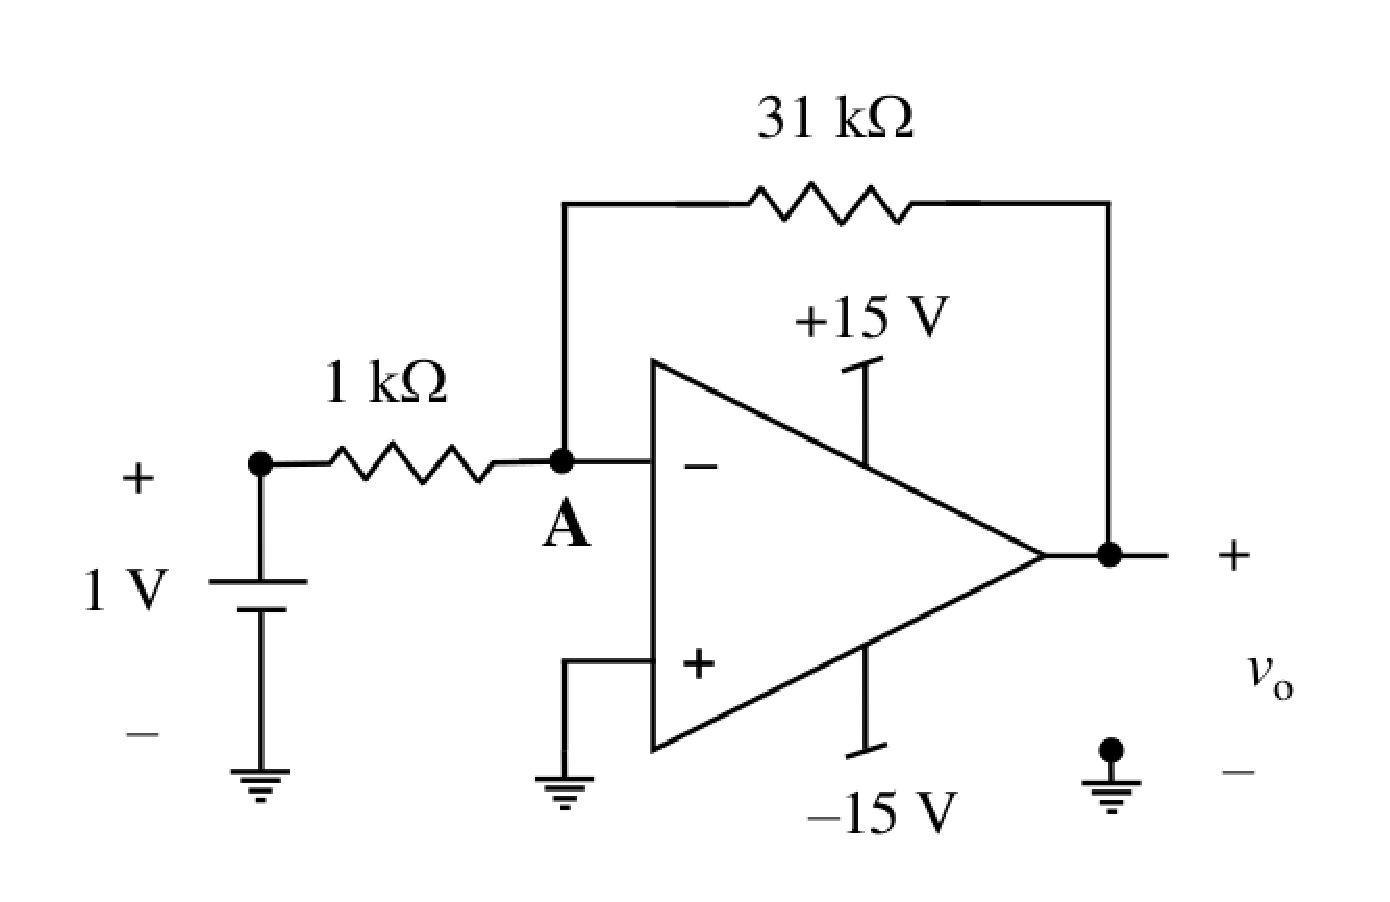
\includegraphics[scale=0.3]{48}

In the above circiut, assume the op-amp to be ideal. The voltage (in volts, correct to one decimal place) at node $A$, connected to the negative input of the op-amp as indicated in the figure is.........

\item The input $4\sin c(2t)$ is fed to a Hilbert trasformer to obtain $y(t)$, as shown in the figure below:

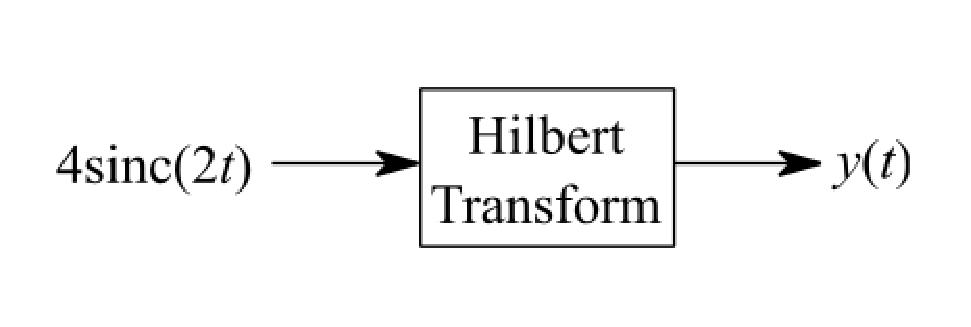
\includegraphics[scale=0.4]{49}

Here $\sin c(x) = \frac{\sin(\pi x)}{\pi x}$. The value(accurate to two decimal places) of
\begin{align*} 
\int_{-\infty}^{\infty}|y(t)|^{2}dt
\end{align*}
is..........

\item A random variable X takes values -0.5 and 0.5 with probabilities $\frac{1}{4}$ and $\frac{3}{4}$, respectively. The noisy observation of X is Y = X + Z. where Z has uniform probability density over the interval (-1, 1). X and Z are independent. If the MAP rule based detector outputs $\hat{X}$ as
then the value of $\alpha$(accurate to two decimal places) is.........

\item For a unity feedback control system with the forward path trasfer function
\begin{align*}
G(s) = \frac{K}{s(s + 2)}
\end{align*}
The peak resonant magnitude $M_r$ of the closed-loop frequency response is 2. The corresponding value of the gain K (correct to two decimal places) is...........

\item The figure below shows the Bode magnitude and phase of a stable trasfer function
\begin{align*}
G(s) = \frac{n_0}{s^3 + d_2s^2 + d_1s + d_0}
\end{align*}

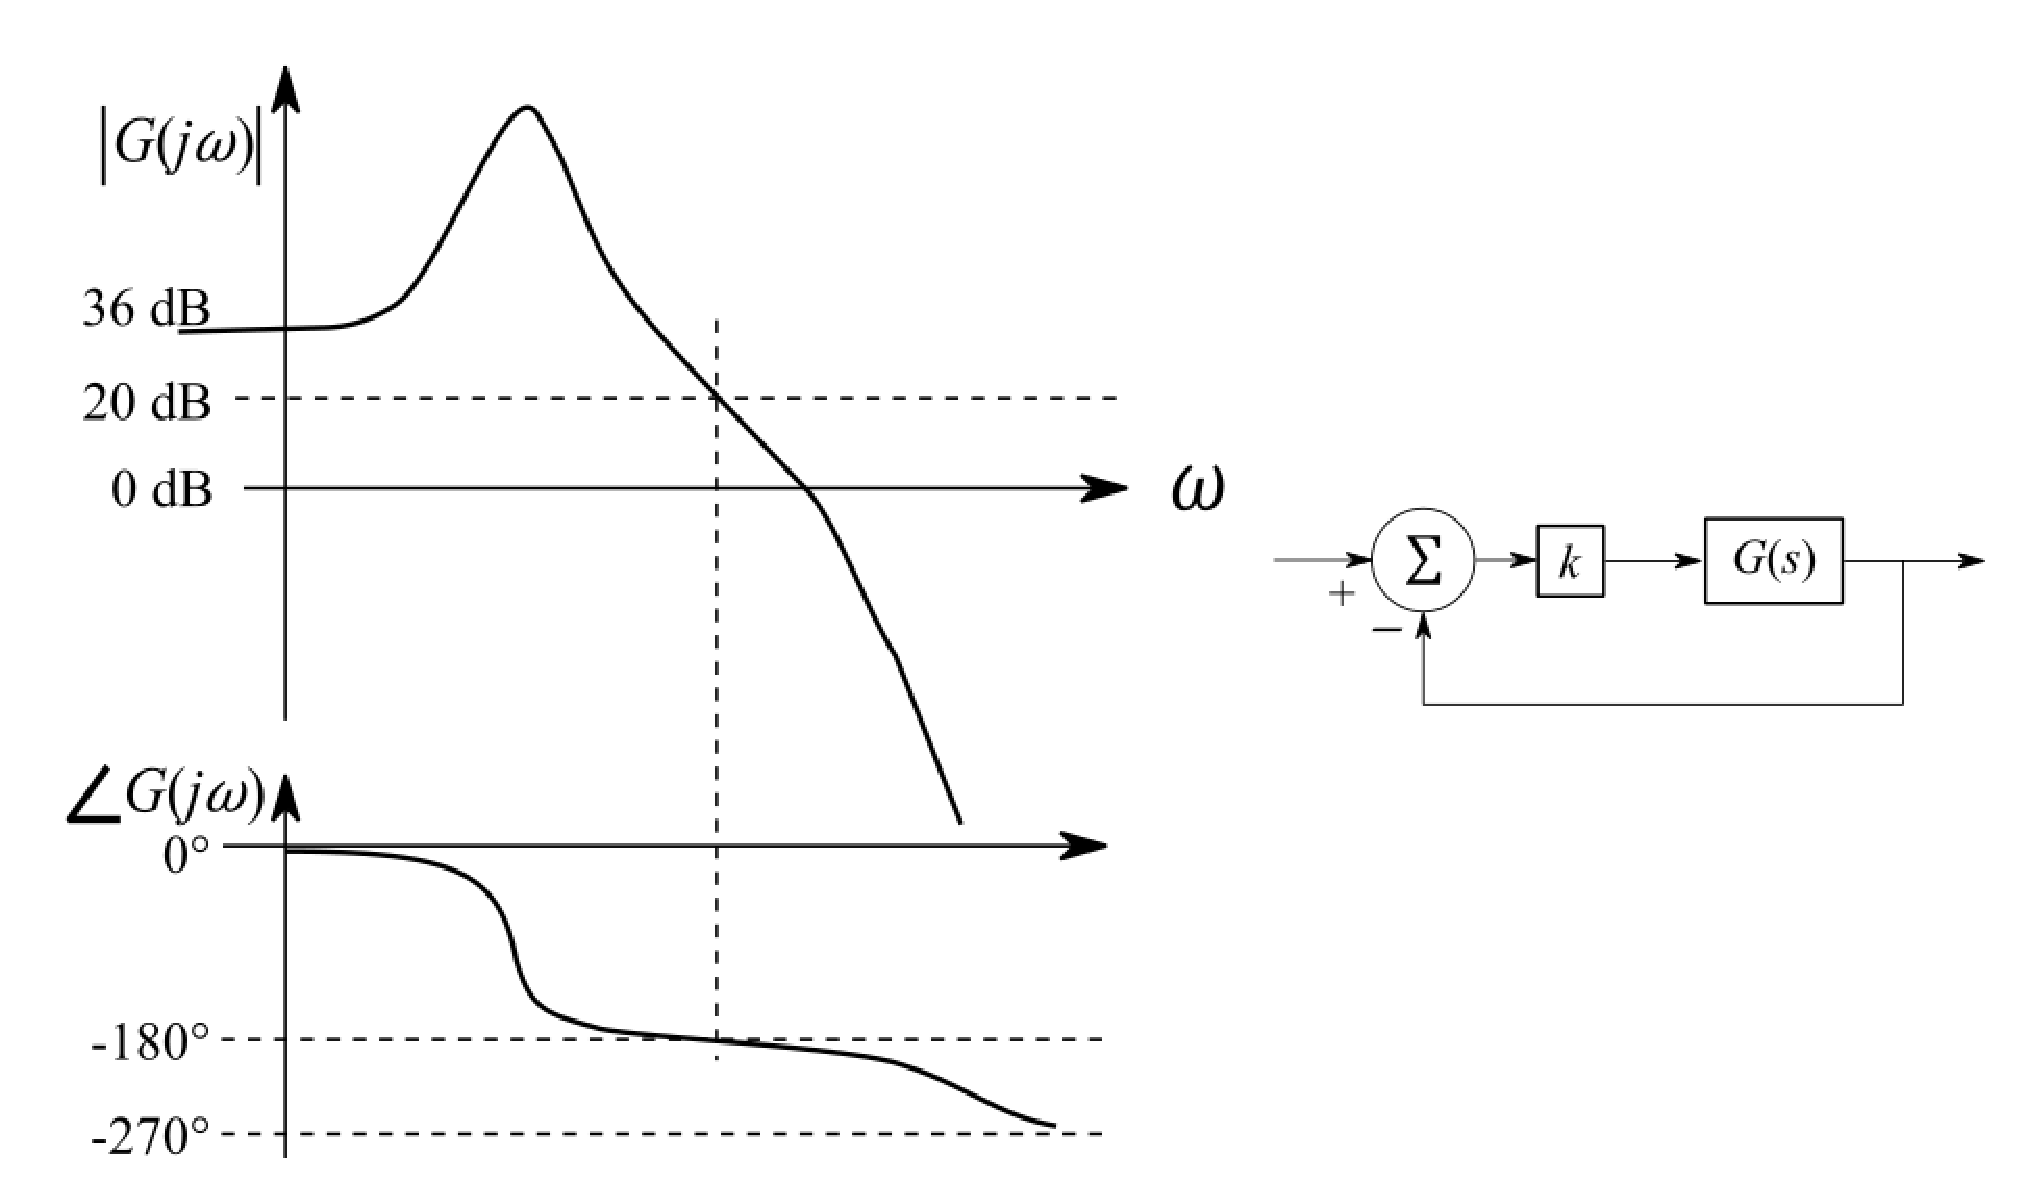
\includegraphics[scale=0.24]{52}

Consider the negative unity feedback configuration with gain k in the feedforward path. The closed loop is stable for 
$k < k_0$. The maximum value of $k_0$ is........

\item In the circuit shown below, the $(W/L)$ value for $M_2$ is twice that for $M_1$. The two nMOS transistors are otherwise identical. The threshold voltage $V_T$ for both transistors is 1.0V. Note that $V_{GS}$ for $M_2$ must be $>$ 1.0V.
Current through the nMOS transistors can be modeled as
\begin{align*}
I_{DS} = \mu C_{ox}\left(\frac{W}{L}\right)\left((V_{GS} - V_T)V_{DS} - \frac{1}{2}V^{2}_{DS}\right)
\end{align*}
\begin{align*}
I_{DS} = \mu C_{ox}\left(\frac{W}{L}\right)\left((V_{GS} - V_T)^{2}/2\right)
\end{align*}

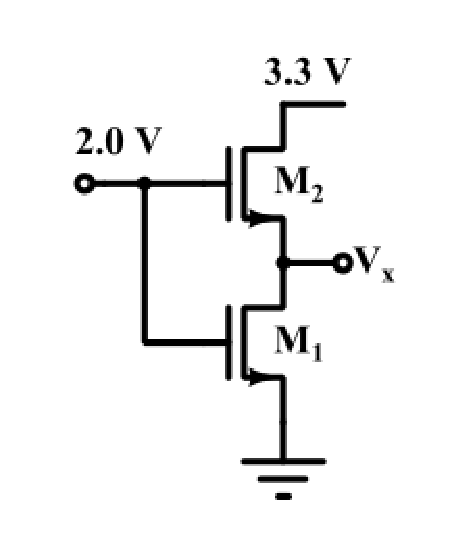
\includegraphics[scale=0.5]{53}

The voltage (in volts, accurate to two decimal places) at $V_x$ is.............

\item A solar cell of area $1cm^2$, operaing at 1.0 sun intensity, has a short circuit current of 20mA, and an open circuit voltage of 0.65V. Assuming room temperature operaion and thermal equivalent voltage of 26mV, the open circuit voltage (in volts, correct to two decimal places) at 0.2 sun intensity is..........

\item A junction is made between $p^{-}Si$ with doping density $N_{A1} = 10^{15}cm^{-3}$ and p $Si$ with doping density 
$N_{A2} = 10^{17}cm^{-3}$.\\
Given: Boltzman constant $k = 1.38 \times 10^{-23}J.K^{-1}$, electronic charge $q = 1.6 \times 10^{-19}C$. Assume $100\%$ acceptor ionization.\\
At room temperature(T = 300K), the magnitude of the built-in potantial(in volts, correct to two decimal places) across this junction will be.............

\item In the circuit shown below, a positive edge-triggered D Flip-Flop is used for sampling input data $D_{in}$ using clock $CK$. The XOR gate outputs 3.3 volts for logic HIGH and 0 volts for logic LOW levels. The data bit and clock periods are equal and the value of $\Delta T/T_{ck} = 0.15$, where the parameters $\Delta T$ and $T_{ck}$ are shown in the figure. Assume that the Flip-Flop and the XOR gate are ideal.

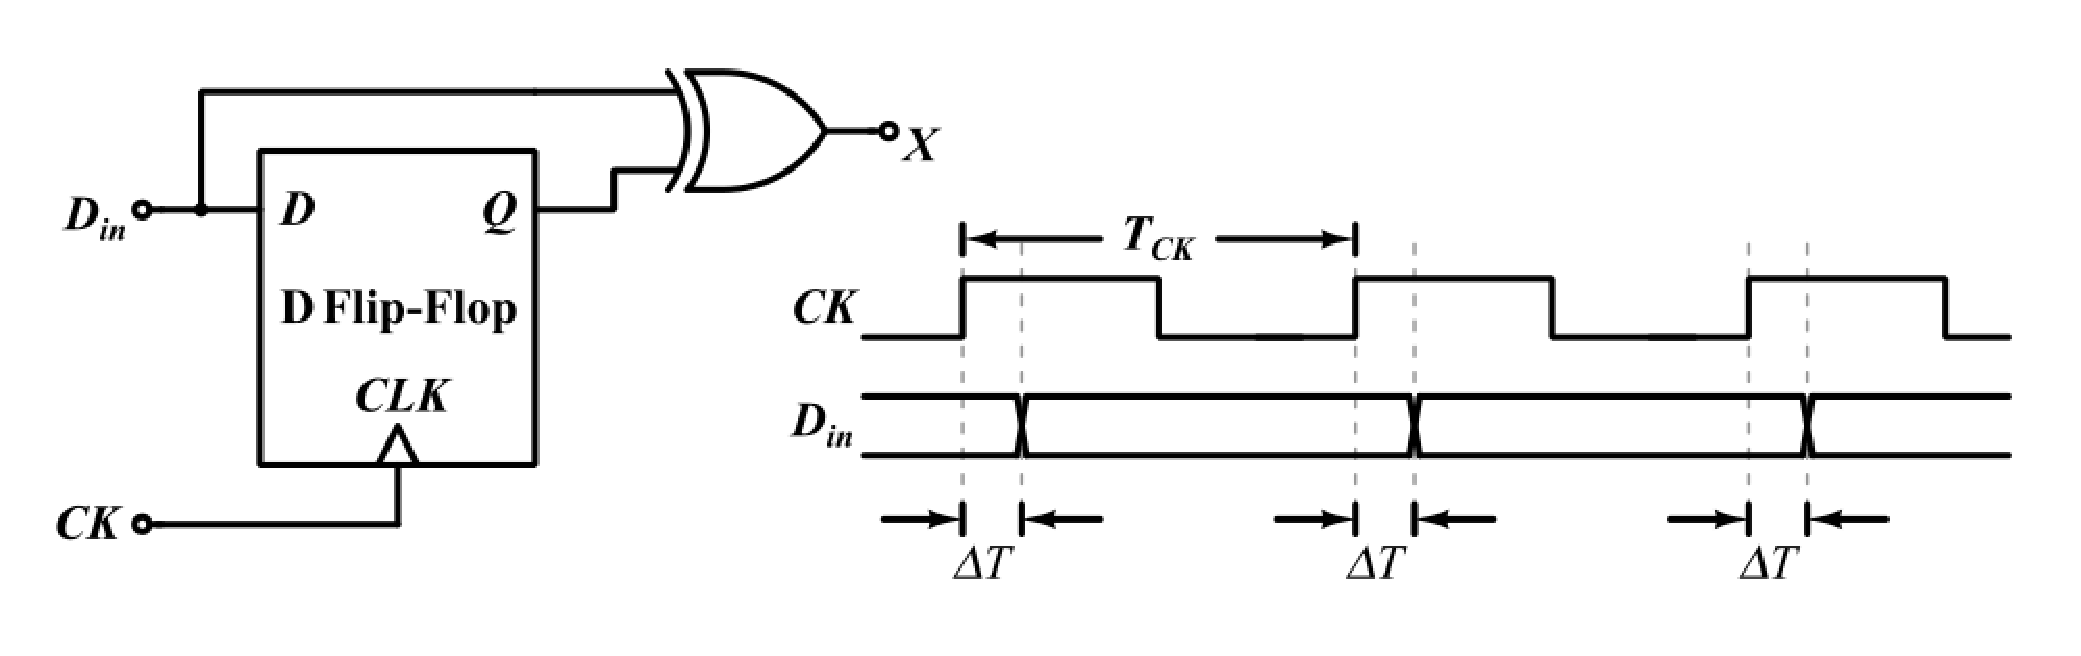
\includegraphics[scale=0.23]{56}

If the probability of input data bit$(D_{in})$ transition in each clock period is 0.3, the average value (in volts, accurate to two decimal places) of the voltage at node X, is..........  

\item The logic gates shown in the digital circuit below use strong pull-down nMOS transistors for LOW logic level at the outputs. When the pull-downs are off, high-value resistors set the output logic levels to HIGH (i.e., the pull-ups are weak). NOte that some nodes are intentonally shorted to implement wired logic. Such shorted nodeswill be HIGH only if the outputs of all the gates whose outputs are shorted are HIGH.

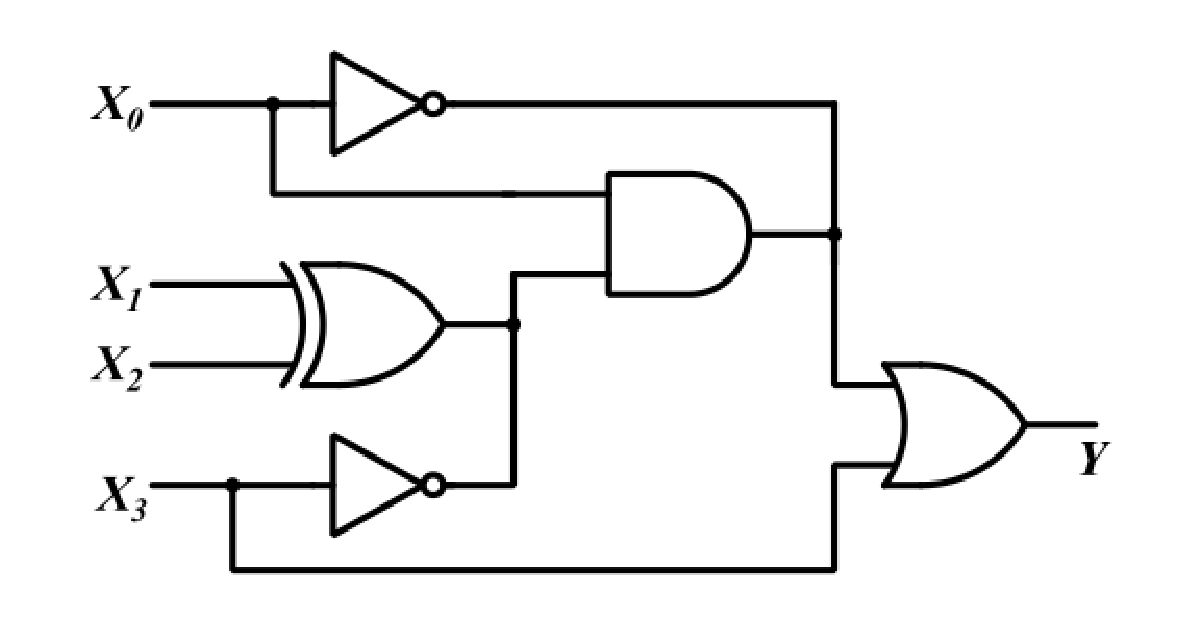
\includegraphics[scale=0.4]{57}

The number of distinct values of $X_3 X_2 X_1 X_0$ (out of the 16 possible values) that give Y = 1 is..........

\item The cutoff frequency of $TE_{01}$ mode of an air filled rectangular waveguide having inner dimensions $a \times b$ $(a > b)$ is twice that of the dominant $TE_{10}$ mode. When the waveguide is operated at a frequency which is $25\%$ higher than the cutoff frequency of the dominant mode, the guide wavelength is found to be 4cm. The value of b (in cm, correct to two decimal places) is......

\item A uniform plane wave traveling in free space and having the electric field
\begin{align*}
\overrightarrow{E}=(\sqrt{2}\hat{a}_{x}-\hat{a}_{z})\cos[6\sqrt{3}\pi \times 10^{8}t-2\pi(x+\sqrt{2}z)]
\end{align*}
is consider on a dielectric medium(relative permittivity $>$ 1, relative permeability = 1)as shown in the figure and there is no reflected wave.

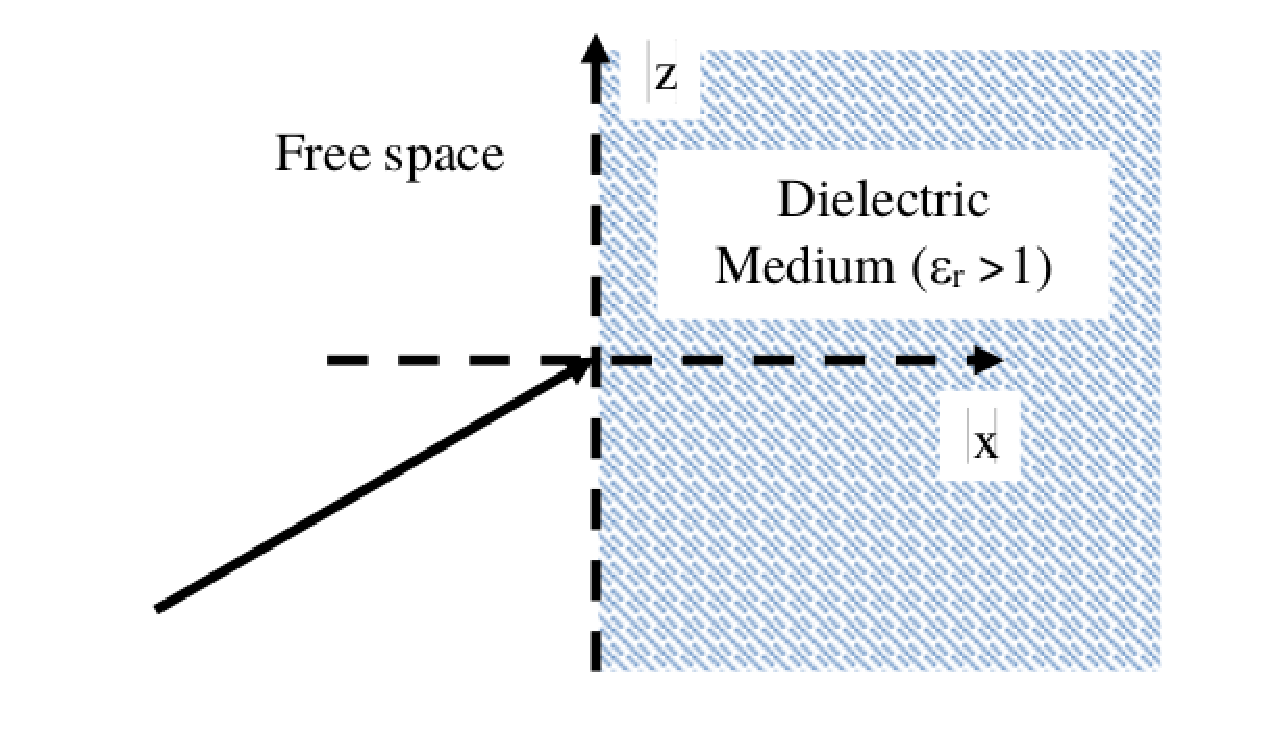
\includegraphics[scale=0.38]{59}

The relative permittivity (correct to two decimal places) of the dielectric medium is...........

\item The position of a particle $y(t)$ is described by the differential equation:
\begin{align}
\frac{d^2y}{dt^2} = -\frac{dy}{dx} - \frac{5y}{4}
\end{align}
The initial conditions are $y(0) = 1$ and $\frac{dy}{dx}_{t = 0} = 0$. The position (accurate to two decimal places) of the particlenat $t = \pi$ is.............

\item The contour C given is on the complete plane $x + jy$, where $j = \sqrt{-1}$.

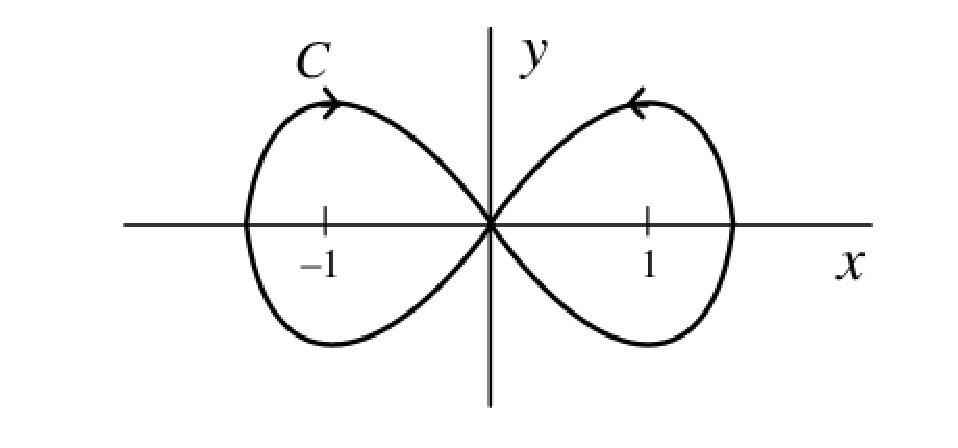
\includegraphics[scale=0.4]{61}

The value of the integral
\begin{align*}
\frac{1}{\pi} \int_{C}\frac{dz}{z^2 - 1}
\end{align*}
is............

\item Let 
\begin{align*}
r = x^2 + y - z
\end{align*}
\begin{align*}
z^3 - xy + yz + y^3 = 1
\end{align*}
Assume that x and y are independent variables. At $(x, y, z) = (2, -1, 1)$, the value (correct to two decimal places) of 
$\frac{\partial r}{\partial x}$ is...........

\item Consider the network shown below with $R_1 = 1\Omega$, $R_2 = 2\Omega$ and $R_3 = 3\Omega$. The network is connected to a constant voltage source of 11V.

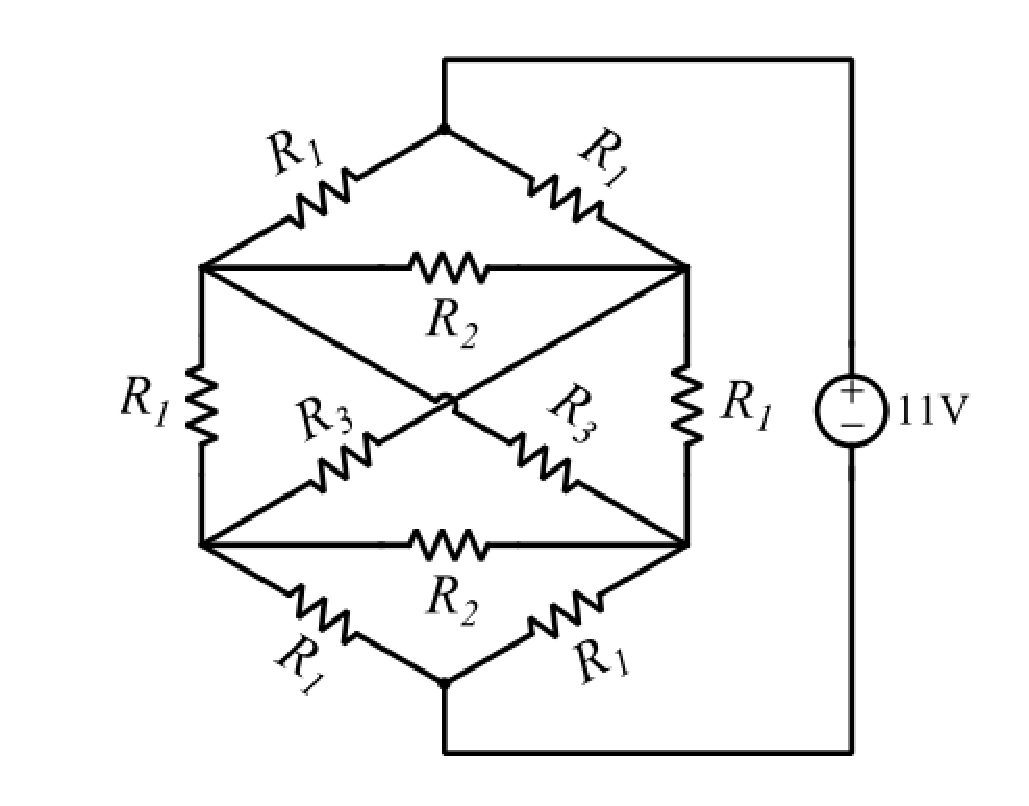
\includegraphics[scale=0.4]{63}

The magnitude of the current (in amperes, accurate to two decimsl places) through the source is............

\item A band limited low-pass signal $x(t)$ of bandwith $5kHz$ is sampled at a sampling rate of $f_s$. The signal $x(t)$ is reconnected using the reconstruction filter $H(f)$ whose magnitude response is shown below:

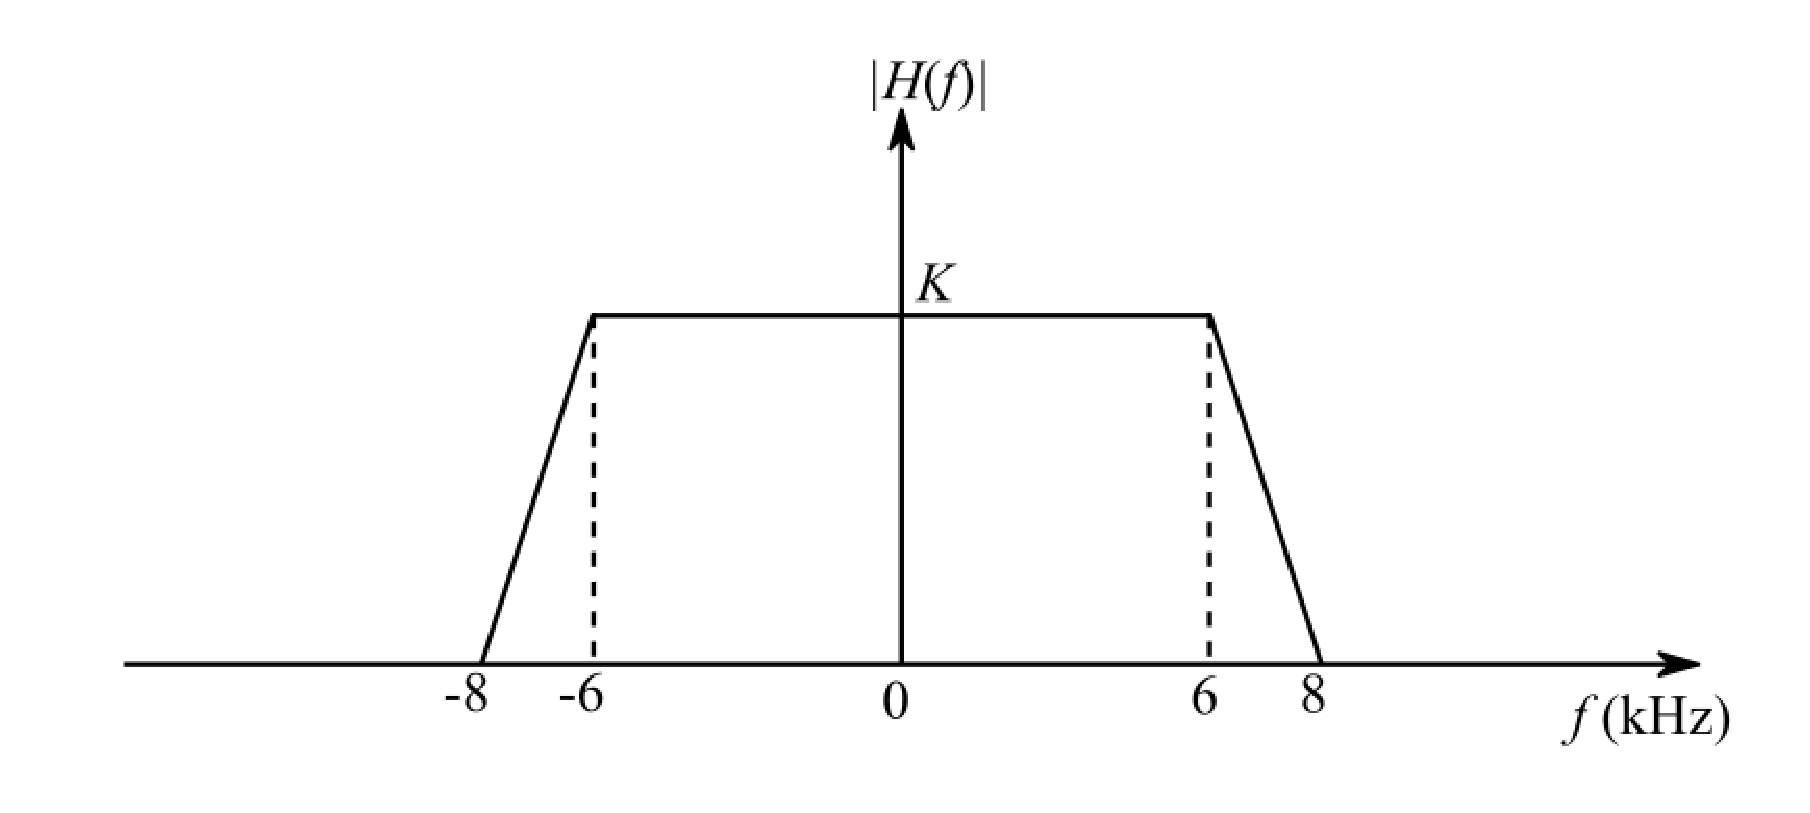
\includegraphics[scale=0.27]{64}

The minimum sampling rate $f_s(kHz)$ for perfect reconstruction of $x(t)$ is..........

\item Let
\begin{align*}
X[k] = k + 1, 0 \leq k \leq 7
\end{align*}
8-point DFT of a sequence $x[n]$, where
\begin{align*}
X[k] = \sum_{n=0}^{N-1}x[n]e^{-j2\pi nk/N}
\end{align*}
The value (correct to two decimal places) of $\sum_{n=0}^{3}x[2n]$ is...........